
\chapter{Cryptanalysis of GOST}\label{ch:GOST}
%cryptoeprint:2007:024
%DEScourtois
%courtois2008algebraicKeeLoq

\section{GOST encryption standard}
The Russian encryption standard
GOST 28147-89 %was developed in the 1970s
is an important government standard
\cite{gost198928147}.
Its large key size of 256 bits
make GOST a plausible alternative for AES-256
and 3-key triple DES.
%% full version maybe %%The latter for the same block size of 64 bits offers keys of only 168 bits.
Clearly GOST is a serious cipher for serious applications
%% full version maybe %%designed with most serious applications in mind.
and at least two sets of GOST S-boxes have been explicitly identified
as being used by the most prominent Russian banks, %financial institutions
cf. \cite{schneier2007applied,GOSTRussianReferenceImplementation}.

The most complete current reference implementation of GOST in OpenSSL library contains eight standard sets of S-boxes
\cite{GOSTRussianReferenceImplementation}. The attacks we consider in this Chapter, work with a very similar complexity for any S-boxes. % used in GOST.

\subsection{GOST And ISO Standardisation.}
The cost of cryptography is still an important problem for the industry,
for example only around 2010 Intel implemented an encryption algorithm
in some of its CPUs, and not yet in all of its CPUs.
It is therefore very important to notice that
in addition to the very long bit keys
GOST has a much lower implementation cost
than AES or any other comparable encryption algorithm.
For example in hardware GOST 256 bits requires less than 800 GE,
while AES-128 requires 3100 GE, see \cite{PoschmannImplement}.
Thus it is not surprising that GOST became an Internet standard,
it is part of many crypto libraries such as OpenSSL
\cite{GOSTRussianReferenceImplementation}, %,Crypto++},
and is increasingly popular %and used
also outside its country of origin
\cite{PoschmannImplement}.
Hard to think about a better algorithm for the industry
with its ultra-low implementation cost and
20 years of cryptanalysis efforts behind it \cite{PoschmannImplement}.
In 2010 GOST was submitted to ISO 18033
to become a worldwide encryption standard.
Less than 10
%Only eight
block ciphers have ever become an
ISO %international
standard.
Unhappily in 2011 several key recovery attacks on GOST have been found
\cite{JapaneseGOSTMITMFSE2011,gostreport,gostac,gostdc0,gostdc2}.

\subsection{Cryptanalysis of GOST}

The turning point in the security of GOST was the discovery of the so called
``Reflection'' property \cite{GOSTReflectionKara}.
Initially at Indocrypt 2008 only a weak-key attack with time complexity of $2^{192}$
is proposed, with large proportion of $2^{-32}$ of weak keys.
Then in 2011 several attacks on regular GOST keys have been discovered,
and more than half of these new attacks use this reflection property \cite{JapaneseGOSTMITMFSE2011,DunkelmanImprovedGOST8R}, sometimes twice, three or four times \cite{gostac}.
Most these attacks can be described as attacks with a ``Complexity Reduction''
\cite{gostreport,gostac} where from
some data for the full 32 rounds GOST we obtain a certain number
of pairs for 8 or less rounds of GOST.
The quantity of data available after reduction is very small,
for example 2,3 or 4 pairs for a reduced cipher.
In this paper we look precisely at questions
pertaining to cryptanalysing 8 rounds GOST with 2,3,4 KP
needed as a last step in numerous already known attacks on GOST
\cite{gostreport,gostac,gostlow8r}.

Many attacks which do not use any reflections
have also been proposed \cite{gostac,gostreport,DunkelmanImprovedGOST8R}
and also differential attacks which do not
fall into the ``Complexity Reduction'' category.
The most recent advanced differential attack on GOST
has time complexity of $2^{178}$, see \cite{gostdc0,gostdc2}
which also the best single-key attack known.

\section{The Internal Structure of GOST}
GOST is a block cipher with a simple Feistel structure,
64-bit block size, 256-bit keys and 32 rounds.
Each round contains a key addition modulo $2^{32}$,
a set of 8 bijective S-boxes on 4 bits,
and a simple rotation by 11 positions.

GOST has 32 identical rounds such as the one described on Fig. \ref{GostRoundAndConnections} below.
They differ only by the subsets of 32 key bits which they use. GOST has a weak key schedule which is the main source of all the attacks on full 32-round GOST \cite{gostreport,gostac,JapaneseGOSTMITMFSE2011,gostdcpp1,gostdc0,gostdc1,gostdc2,DunkelmanImprovedGOST8R}. 
In this paper however we only look at up to 8 rounds of GOST which have independent 32-bit keys which don't repeat, therefore we can ignore the GOST key scheduling totally.

We number the inputs of the S-box Si for $i=1,2,\ldots,8$ by integers from $4i+1$ to $4i+4$ out of $1..32$ and its outputs are numbered according to their final positions after the rotation by 11 positions: for example the inputs of S6 are $20,21,22,23$ and the outputs are $32,1,2,3$.


\begin{figure}[h]
	\centering
	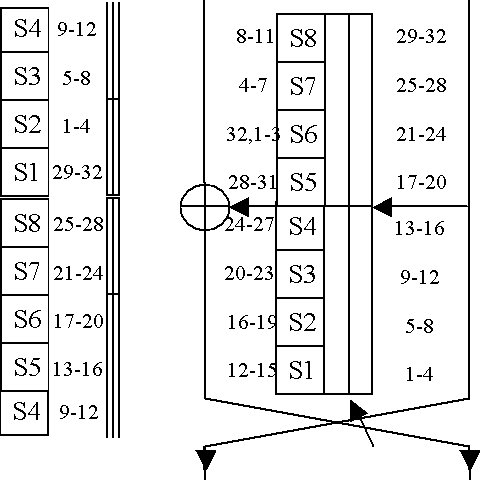
\includegraphics[width=60mm]{./pics/gostfeist2.jpg}

	\caption{One Round of GOST And Connections in The Following Round}
	\label{GostRoundAndConnections}
\end{figure}



On our picture %below
Fig. \ref{GostRoundAndConnections}
the $\boxplus$ denotes the addition modulo $2^{32}$.
At the left margin
on Fig. \ref{GostRoundAndConnections}
we also show S-box numbers
in the next round,
which is very helpful,
to see which bits are successfully determined
in our attacks on GOST.
In a great simplification,
in most cases,
one S-box in one round affects essentially
only two consecutive S-boxes in the next round.
Additional propagation is obtained due to the Feistel structure
and due to carries in the modular addition.

\section{Algebraic Cryptanalysis with Complexity Reduction}

Following \cite{gostreport,gostac}
the work of cryptanalyst
who wants to cryptanalyse GOST
can be split into two independent tasks.
First task is how to achieve a software algebraic attack
on a reduced-round version
as discussed in the previous section.
The second question is if and {\bf how}
the complexity major variants of full GOST with 32 rounds
can ever be {\bf reduced}
to a problem of breaking a cipher with much less rounds.
In fact only in the recent 5 years
it became possible to design and implement
an appropriate last step
for many such attacks
which is a software algebraic attack,
a Meet-In-the-Middle (MITM) attack, or other low-data complexity attack.
This last step is the main focus in this paper.


\subsection{Reductions and Black-Box Reductions}


The main idea is as follows \cite{gostreport,gostac}:
In order to reduce the attack complexity,
we exploit the self-similarity of the cipher
(due for example to a weak key schedule)
and add some well-chosen assumptions which produce interesting
and sometimes quite non-trivial consequences
due to the high-level structural properties of the cipher,
which makes cryptanalysis problems
smaller, simpler and easier to solve.
In this process we need to minimise the costs
(in terms of probability that our assumptions hold)
and to maximise the benefits
(in terms of the number and the complexity of interesting relations
which hold under these assumptions).

This process is called
{\bf Algebraic Complexity Reduction},
see \cite{gostreport,gostac}.
In most cases what we get is to compute (guess or determine)
many internal values inside one or several decryptions,
and literally break the cipher apart into smaller pieces.
In particular we have
{\bf Black-Box Algebraic Complexity Reductions}
where we obtain real black-box reductions,
to for example the same cipher with strictly less rounds
(and less data)
again at the cost of some well-chosen assumptions.
Most but not all reductions we are aware of
are real ``black box'' reductions, see \cite{gostac}
for a detailed discussion.
The
notion of
Algebraic Complexity Reduction
creates
new important {\bf optimisation problems}
in symmetric cryptanalysis:
which deals with the fundamental question
of how we can reduce the complexity
of a cipher in cryptanalysis
to a simpler problem,
with a limited quantity of data,
and with greatly reduced complexity,
and this in the best possible (optimal)
way while many interesting and non-trivial
solutions will exist.
One example of a
Black-Box Algebraic Complexity Reduction
from $2^{64}$ KP for 32 rounds of GOST,
to 4 KP for 8 rounds of GOST, can be found in \cite{gostreport}
and many more in \cite{gostac}.

Algebraic Complexity Reduction is a sort of umbrella paradigm
which generalizes many already known
fixed point, sliding, reflection and involution attacks.
One is able to exploit similarities
of individual sub-blocks and their inverses.
We have reflection attacks \cite{GOSTReflectionKara}
but also have new attacks
with double triple and quadruple reflection \cite{gostac}.
We are able to relax the conditions
necessary in slide attacks
\cite{slide2} in nearly arbitrary ways.
We have many new sort of self-similarity attacks, cf. \cite{gostac}.
though reflection attacks \cite{GOSTReflectionKara,gostac}
are related to fixed point attacks which are
an important attack for ciphers
with block size being smaller than the key size, cf.
\cite{courtois2008algebraicKeeLoq,KeeLoqTatra}.




\subsection{Optimizing The Reductions: Amplification}


Reductions can be compared in terms of the number of pairs obtained, the resulting reduced number of rounds, success probability, and in terms of plaintext complexity, see \cite{gostac,gostreport}.
A key property
of these reductions
is the process of so called {\bf Amplification}
which was introduced in \cite{AlgSnowCourtoisDebraize}.

\begin{mydef}[Amplification, Informal]
	The goal of the attacker
	is to find a reduction where he makes some assumptions
	at a certain initial cost,
	for example they are true with probability $2^{-X}$
	or work for certain proportion $2^{-Z}$ of keys.
	Then the attacker can in constant time determine
	many other internal bits inside the cipher to the total of $Y$ bits.
	
	We are only interested in cases in which the values
	$X$ and $Z$ are judged realistic for a given attack,
	for example $Z<32$ and $X<128$.
	
	We call amplification the ratio $A=Y/X$.
\end{mydef}

The amplification is an important question in algebraic cryptanalysis
which was previously discussed in
\cite{AlgSnowCourtoisDebraize}.
We should note that there are some difficulties in defining this ratio formally:

\begin{enumerate}
	\item
	We claim that we need specific definitions for each individual cipher and
	for each specific attack method.
	For example $Y$ can be the total number of linear equations obtained with the ElimLin
	algorithm \cite{AlgSnowCourtoisDebraize,DEScourtois,ElimLinR}
	after adding a well-chosen set of
	$X$ linear equations on the internal bits inside the cipher.
	
	\item
	Intuitively,
	the higher, this amplification coefficient $A$ is,
	while $X$ and $Z$ remain below a certain threshold,
	the stronger and more surprising is the attack obtained.
	
	\item
	With higher  values of $X$, the amplification can also be higher,
	however the attacker must limit the size of $X$
	for the whole the attack to remain fast enough overall.
	
	\item
	It is very difficult to know if an attack with given parameters may exist.
\end{enumerate}


{\bf Examples.}
In the most basic slide attack based on periodicity
in the key scheduling \cite{slide2}
the amplification is unlimited.
From one ``slid pair'', we can obtain another ``slid pair'',
then another, etc..
However in more advanced sliding attacks which operate with imperfect
periodicity, the amplification can be limited, or occur only after the attacker
guesses a few key bits, see \cite{courtois2008algebraicKeeLoq,KeeLoqTatra}.

Another example where the amplification is exceptionally high is the Weak Key Family 3 in \cite{gostac}.
In this case the amplification is very very high: $X=1$ and $Y=256$
while $Z=64$, see \cite{gostac}.
This can only be obtained for some weak keys in GOST with $Z=64$.
In spite of the additional of factor of $2^{64}$ implied by this value of $Z$
the amplification is very high
and overall it leads to very efficient attacks on certain GOST keys,
see \cite{gostlow8r,gostac}.
The work described in this chapter is mostly motivated
by the question how one can identify
the suitable sets of key bits for such attacks.


\subsection{Working at The Low Level}

The amplification is easy to define as in many initial steps in the cryptanalysis of GOST \cite{gostac}, we deal with black boxes.
It is harder but possible to define at the low level, when we look at a complete functional description of a cipher.
Here the question is what is the best possible software attack with tools such as the ElimLin algorithm \cite{AlgSnowCourtoisDebraize,DEScourtois,ElimLinR} SAT solvers \cite{OptimiPaper,BardCourtoiJeffersonConv}, Gr\"{o}bner bases \cite{grobner} and other \cite{SemaevSparseJournalPaper}. In all these algorithms we observe the phenomenon of Amplification in various forms. For example we can study and count linearly independent linear equations and try to amplify their number
by the ElimLin algorithm, see \cite{AlgSnowCourtoisDebraize,DEScourtois,ElimLinR}.
%this is still almost black box: non-linear operations are seen as black boxes... or grey boxes...
%However as previously explained, amplification can become very high.
When the ElimLin algorithm is itself the last step of the attack, or if the SAT solver is the last step of the attack, this amplification phenomenon becomes very important. We observe an avalanche-like phenomenon where more and more new linear equations are generated in the ElimLin algorithm, until the system is solved. Similarly, with SAT solver there is a point of phase transition
where the problem becomes really easy to solve. If we want to understand algebraic cryptanalysis we need precisely to work
on this face transition phenomenon itself. What happens after this threshold when the problem is just very easy to solve
is less important.

Our work focus more specifically on cryptographic attacks with SAT solvers, and on GOST, which is a nice example
of a weak government standard cipher with relatively poor diffusion. There are two main approaches in SAT cryptanalysis
or two main algorithms to break a cipher with a SAT solver:

\begin{enumerate}
	\item
	{\bf The SAT Method:}
	Guess $X$ bits and run a SAT solver which,
	if the assumption on $X$ bits is correct takes time $T$.
	Abort all the other computations at time $T$.
	The total time complexity is about $2^{X}\cdot T$.
	\item
	{\bf The UNSAT Method:}
	Guess $X$ bits and run a SAT solver which,
	if the assumption on $X$ bits is incorrect
	finds a contradiction in time $T$
	with large probability $1-P$ say 99 $\%$.
	
	With a small probability of $P>0$,
	we can guess more key bits
	and either find additional contradictions
	or find the solution.
	
	The idea is that if $P$ is small enough the complexity of
	these additional steps can be less then the $2^{X}\cdot T$ spent
	in the initial UNSAT step.
	
	\item
	{\bf A Mixed UNSAT/SAT Attack:}
	In practice maybe $P$ is not as small as we wish, and therefore we may have
	a mix of SAT and UNSAT method:
	where the final complexity will be a sum of two terms none
	of which can be neglected.
	We will see a very nice example
	how a combined attack can be better
	than any of SAT and UNSAT methods in isolation
	in Section \ref{section:Fact8R4KP_94_SATMethod}.
\end{enumerate}

\subsection{Applications of UNSAT/SAT Immunities}
\noindent 
{\bf Cryptanalysis}. %Intended Application.}
The main idea is that these two numbers will
allow to evaluate the security of the cipher
against cryptanalytic attacks with a SAT solver.
Upper bounds we obtain do translate, more or less, as we will see,
into concrete attacks with complexity of about $2^{X}$.
The two figures will also indicate which of the three
strategies: SAT/UNSAT/Mixed is more likely to work.

\noindent
{\bf Design of Block Ciphers}.
It is easy to see
that the designer of a cipher
can very effectively lower-bound
these quantities.
This will be achieved by making sure
that each S-box in each round
influences as many S-boxes as possible in the next round.
This is not all very different than designing a cipher
which is provably resistant to linear and differential cryptanalysis.
Interestingly,
Schneier once claimed that ``Against differential and linear cryptanalysis, GOST is probably stronger than DES''
\cite{schneier2007applied}.
Therefore we should also expect that Contradiction Immunity
of DES and GOST are comparable.
Happily, similar attacks with SAT solvers have been developed
for both DES \cite{DEScourtois} and GOST \cite{OptimiPaper}.
In fact, it is obvious that the diffusion in DES
is much better than in GOST and so is the Contradiction Immunity in DES.
However we need to be careful about drawing any conclusions
and direct comparisons do not mean much.
If the contradiction immunity is 78 for 8 out of 32 rounds of GOST with 3 KP and 256-bit keys,
is it better or less good,
than contradiction immunity
being 20 for 6 rounds out of 16 of DES with 1 KP and 56-bit keys?
It is very hard to say.

\section{Application to DES}

In this section we give some basic results for DES
obtained by the methods
of \cite{DEScourtois}
with however a better SAT solver
CryptoMiniSat 2.92 \cite{CryptoMiniSat}.
Unhappily in DES the key bits are spread more
or less uniformly in different rounds, and they tend to repeat many times.
Therefore it is difficult to choose really good sets of bits
and for now we just report upper bounds obtained when choosing
the key bits at random, and letting the SAT solver to do the job.

\begin{fact}
	\label{ContrImmDES6Rounds}
	The Contradiction Immunity
	%is at most 28 for 6 rounds of DES and it
	is at most 44 for 8 rounds of DES.
\end{fact}

\begin{fact}
	\label{SATImmDES6Rounds}
	The SAT Immunity
	%is at most 17 for 6 rounds of DES and 1 KP and it
	is at most 34 for 8 rounds of DES and 1 KP.
\end{fact}

These two results were obtained with the gate-efficient encoding described in \cite{DEScourtois}, and with CryptoMiniSat 2.92 \cite{CryptoMiniSat}. We found no attack on 8 rounds of DES and 1 KP which would be faster than brute force. For ultra low-data complexity attacks, 8 rounds of DES seem already secure or secure enough.

\section{Application to GOST}

In this paper we are going to provide some results on the Contradiction Immunity and SAT Immunity of GOST. These results are constructive upper bounds.

For a long time we thought that the Contradiction Immunity of 8 rounds of GOST was about 128.
The reason for that can be found on Fig. 4 in \cite{gostdc2}:
it is possible to see that GOST splits very neatly into
two nearly independent ciphers with 128-bit key each,
which are only loosely connected.
With this idea it is easy to understand why a software/algebraic
attack on 8 rounds of GOST with complexity of $2^{120}$
seems plausible and natural.
%% full version maybe %%, and that we do not expect much faster such attacks to exist.
However recently we found that it is much lower than 128,
much closer to 64.
This was the main motivation for writing this paper.

{\bf Notation, cf. Fig. \ref{Gost81optimal4KPUNSAT78}}:
We denote by $S^{1}3$ just 1 higher ranking bit at S-box 1 in a given round.
Similarly we denote by $S_{3}3$ the 3 lower ranking bits of S3.

\begin{figure}[h]
	\centering
	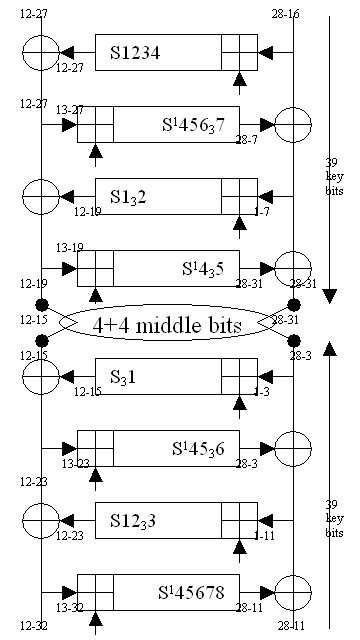
\includegraphics[width=60mm]{./pics/gost81optimal4KP.jpg}
	\caption{Our best set of 78 bits for UNSAT}
	\label{Gost81optimal4KPUNSAT78}
\end{figure}

\begin{fact}
	\label{ContrImm8Rounds}
	The Contradiction Immunity
	for 8 rounds of GOST is at most 78.
\end{fact}

\noindent\emph{Justification:}
We have constructed and tried many different sets aiming at a contradiction in the middle.
Our best set is as follows (cf. Fig. \ref{Gost81optimal4KPUNSAT78}):
0-15,47-58,64-70,111-114,128-130,175-182,192-202,239-255.
The contradictions can be found in time of 0.06 s
with CryptoMiniSat 2.92 software \cite{CryptoMiniSat}
with probability of about 50 $\%$.
It is easy to see that they could be obtained in essentially constant time
by a dedicated algorithm with some small precomputed tables.

{\bf Remark.}
In fact we come remarkably close to 68 bits.
If we consider the set of 68 bits
later shown on Fig \ref{Gost81optimal4KPSAT68Bits}
and also used in \cite{gostlow8r},
we we achieve about 39 $\%$ UNSAT with CryptoMiniSat 2.92.
It is remarkably close but it does not achieve 50 $\%$ required.
This may seem strange, but in order to achieve 50 $\%$,
many more key bits are needed, cf. Fact \ref{ContrImm8Rounds} above.
This is because in GOST it makes a lot of sense to guess key bits
for full S-boxes, and S-boxes active in one round
call for other S-boxes being also active.

\subsection{SAT Immunity of GOST}
Unhappily, it turns out that a set which is good for UNSAT is
typically NOT good at SAT.
No SAT solver software we dispose of is able to find the missing
bits if the 78 bits of Fig. \ref{Gost81optimal4KPUNSAT78} are fixed.
Happily we have found sets which are very good at SAT
and they are in fact smaller than 78.
Our best result is as follows:


\begin{fact}
	\label{SATImm8Rounds}
	The SAT Immunity
	for 8 rounds of GOST and 4 KP
	is at most 68.
\end{fact}


\noindent\emph{Justification:}
We use the following set of bits
depicted on Fig \ref{Gost81optimal4KPSAT68Bits}
0-15,51-55,64-66,128-130,179-183,192-207,224-231,244-255
which is also used in \cite{gostlow8r}.
All the remaining 256-68 bits can be determined in time of
about 400 seconds
using GOST encodings described in \cite{optisharcs}
and with CryptoMiniSat 2.92 \cite{CryptoMiniSat}.

From here a naive ``SAT strategy'' attack on GOST would be to run
a SAT solver for 400 seconds $2^{68}$ times.
This would be about $2^{99}$ GOST encryptions.


\begin{figure}[h]
	\centering
	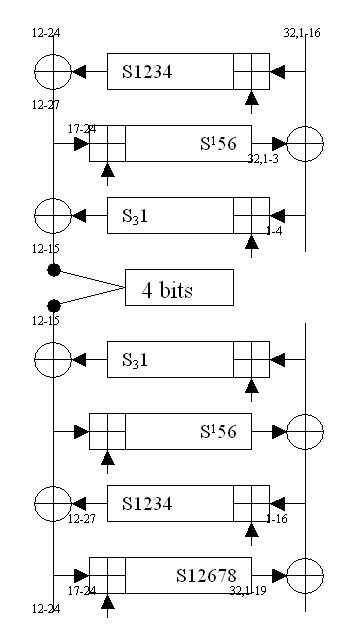
\includegraphics[width=60mm]{./pics/gost81optimalSAT4KP.jpg}
	\caption{Our best set of 68 bits for SAT}
	\label{Gost81optimal4KPSAT68Bits}
\end{figure}

{\bf Further Improvement.}
In order to improve this attack,
the interesting question is if we
can obtain contradictions when one of the  $2^{68}$ cases is incorrect,
and for what proportion of cases, and how long would it take.
In other terms, we would like our set of 68 bits
or possibly a smaller subset, to be good at UNSAT, which is the case as we have
previously seen.
In our attack with 4 KP
we want to find a contradiction
for all the 4 pairs simultaneously.
This will be easier than contradiction with 1 KP
we studied previously.
This leads to the following improved attack
which mixes the SAT and UNSAT strategies
and which is also described in \cite{gostlow8r}.


%\newpage

\vskip-9pt
\vskip-9pt
\section{A Mixed Attack with 4 KP}
\label{section:Fact8R4KP_94_SATMethod}
\vskip-5pt

\begin{fact}
	\label{Fact8R4KP_94_SATMethod}
	Given 4 KP for 8 rounds of GOST
	the full 256-bit key can be found in
	time of about $2^{94}$
	GOST computations and negligible memory.
\end{fact}

\noindent\emph{Justification:}
As in \cite{gostlow8r} we proceed as follows.

%\vskip-4pt
%\vskip-4pt
\begin{enumerate}
	\item
	We use our set of 68 bits as
	on Fig \ref{Gost81optimal4KPSAT68Bits}. %and in Fact \ref{SATImm8Rounds}.
	\item
	We run the software $2^{68}$ times for all possible assignments of the 68 bits.
	\item
	Computer simulations
	with the timeout of 7 seconds,
	a proportion of $1-2^{-5}$ of cases on 68 bits terminates with UNSAT
	within 2 s on average.
	\item
	Overall, we only need to run a proportion of $2^{-5}$ of all the $2^{68}$ cases
	for as many as 400 seconds,
	in other cases it simply terminates automatically within 2 s
	which is $2^{23}$ GOST encryptions on the same CPU.
	\item
	Assuming that all the other cases run for 400 s (some still terminate earlier)
	our conservative estimate of the attack time is
	$2^{68+23}+2^{68+31-5}\approx 2^{94}$ GOST computations.
\end{enumerate}

\subsection{Application to Full 32-round GOST}


Following \cite{gostlow8r,gostac},
this can be transformed into an attack on GOST in the multiple key scenario.
If there is
a suitable %comparably not unrealistic
population of at least $2^{64}$ different keys generated at random,
then one can find one valid 256-bit key,
in time of about $2^{94}$ GOST encryptions for one (weaker) key.
This can be converted into attacks on full GOST not in just one way,
on the contrary there are tens of ways of doing it
which is outside of the scope of this paper,
we refer to \cite{gostreport,gostlow8r,gostac}. %for additional details.

